% !TEX root = main.tex
\section{Spettro delle Ampiezze e delle Fasi}

Nella presente sezione si calcolano e figurano le prime 10 armoniche positive del segnale $y(t)$, partendo dall'equazione formale sviluppata nel capitolo precedente.

Dal calcolo numerico dei coefficienti, ricordando che la frequenza fondamentale è $f_0 = 1/T_0 = 6\text{ kHz}$ e sostituendo i valori nell'espressione trovata:
\begin{align*}
    Y_0 &= 2.25 \text{ V} \\
    Y_{2m} &= 0 \\
    Y_{2m+1} &= \frac{6}{\pi^2 k^2} + \frac{3}{2 \pi k} \sin\left(k \frac{\pi}{2}\right) \text{ V}
\end{align*}
si deducono i valori tabulati di seguito. \textit{Nota bene:} Si ricorda che per ricostruire un segnale dalla propria serie di Fourier trigonometrica, l'ampiezza di ciascuna cosinusoide armonica (da inserire eventualmente in un simulatore come GNU Radio) ammonta al doppio del modulo del coefficiente complesso esponenziale ($2|Y_k|$), ad eccezione della componente continua.

\begin{table}[h]
\centering
\begin{tabular}{|c|c|c|c|c|}
\hline
\textbf{Armonica n° ($k$)} & \textbf{Coefficiente $Y_k$} & \textbf{Frequenza [kHz]} & \textbf{Ampiezza $2|Y_k|$ [V]} & \textbf{Fase $\vartheta_k$ [rad]} \\
\hline
0 & 2.2500 & 0 & 2.2500 & 0 \\
1 & 1.0854 & 6 & 2.1708 & 0 \\
2 & 0 & 12 & 0 & 0 \\
3 & -0.0917 & 18 & 0.1833 & $\pi$ \\
4 & 0 & 24 & 0 & 0 \\
5 & 0.1198 & 30 & 0.2396 & 0 \\
6 & 0 & 36 & 0 & 0 \\
7 & -0.0558 & 42 & 0.1116 & $\pi$ \\
8 & 0 & 48 & 0 & 0 \\
9 & 0.0606 & 54 & 0.1211 & 0 \\
10 & 0 & 60 & 0 & 0 \\
\hline
\end{tabular}
\caption{Valori spettrali delle prime 10 armoniche positive}
\end{table}

\subsection{Grafici dello Spettro}
Di seguito sono mostrati, in forma di spettri a righe (tipici dei segnali periodici), gli andamenti dell'ampiezza $|Y_k|$ e della fase $\angle Y_k$ calcolati numericamente in scala.

\vspace{0.5cm}

\begin{center}
\begin{minipage}{0.48\textwidth}
\centering
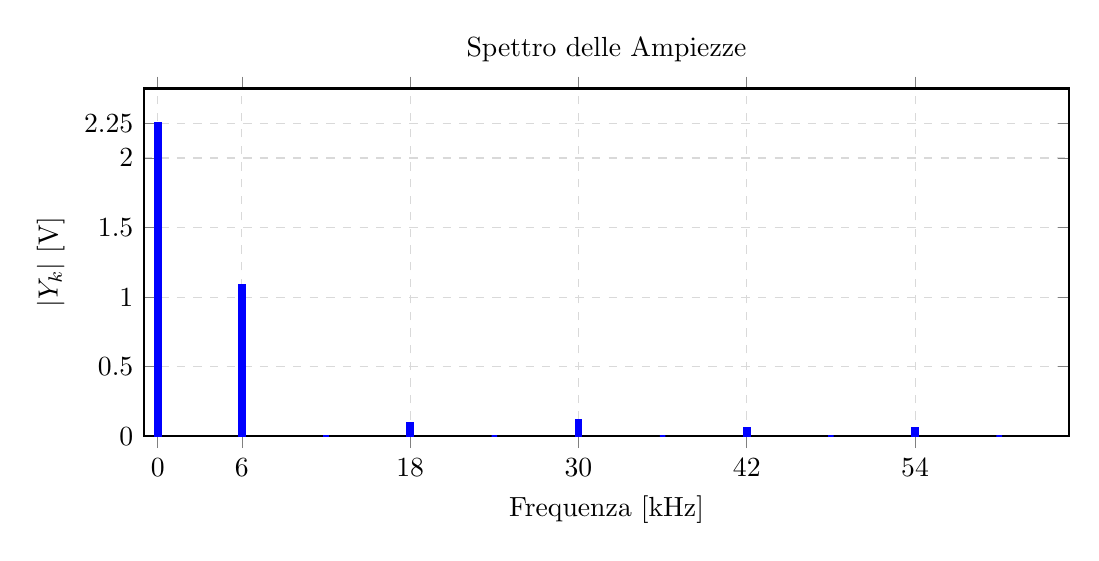
\begin{tikzpicture}
\begin{axis}[
    width=1.1\textwidth,
    height=6cm,
    ymin=0, ymax=2.5,
    xmin=-1, xmax=65,
    xlabel={Frequenza [kHz]},
    ylabel={$|Y_k|$ [V]},
    ybar,
    bar width=2pt,
    grid=both,
    grid style={dashed, gray!30},
    thick,
    xtick={0, 6, 18, 30, 42, 54},
    ytick={0, 0.5, 1, 1.5, 2, 2.25},
    title={Spettro delle Ampiezze}
]
\addplot[color=blue, fill=blue] coordinates {
    (0, 2.25)
    (6, 1.0854)
    (12, 0)
    (18, 0.0917)
    (24, 0)
    (30, 0.1198)
    (36, 0)
    (42, 0.0558)
    (48, 0)
    (54, 0.0606)
    (60, 0)
};
\end{axis}
\end{tikzpicture}
\end{minipage}
\hfill
\begin{minipage}{0.48\textwidth}
\centering
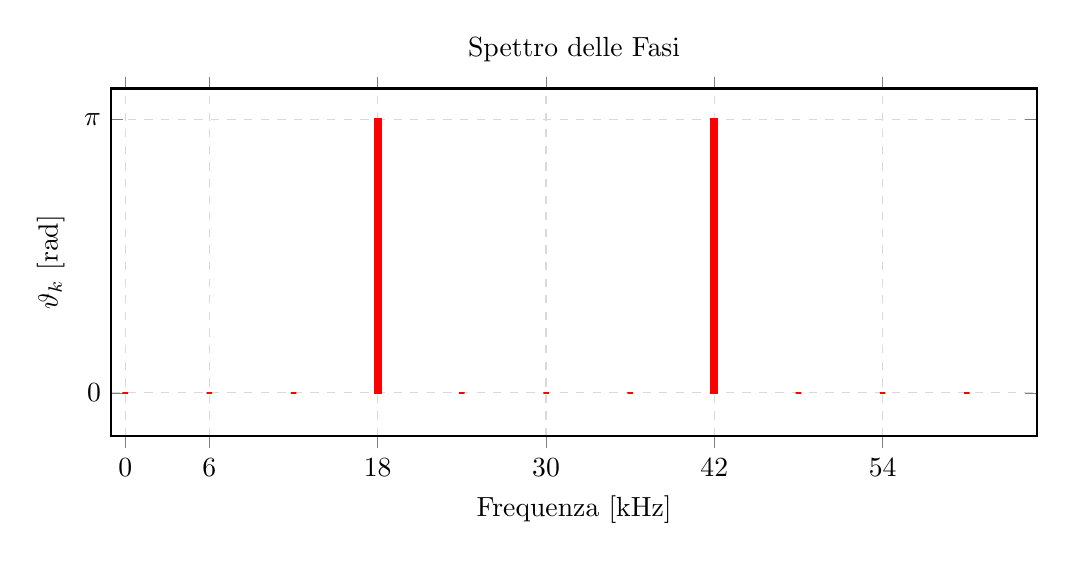
\begin{tikzpicture}
\begin{axis}[
    width=1.1\textwidth,
    height=6cm,
    ymin=-0.5, ymax=3.5,
    xmin=-1, xmax=65,
    xlabel={Frequenza [kHz]},
    ylabel={$\vartheta_k$ [rad]},
    ybar,
    bar width=2pt,
    grid=both,
    grid style={dashed, gray!30},
    thick,
    xtick={0, 6, 18, 30, 42, 54},
    ytick={0, 3.14159},
    yticklabels={0, $\pi$},
    title={Spettro delle Fasi}
]
\addplot[color=red, fill=red] coordinates {
    (0, 0)
    (6, 0)
    (12, 0)
    (18, 3.14159)
    (24, 0)
    (30, 0)
    (36, 0)
    (42, 3.14159)
    (48, 0)
    (54, 0)
    (60, 0)
};
\end{axis}
\end{tikzpicture}
\end{minipage}
\end{center}

Come si può notare, lo spettro di fase balza coerentemente a $\pi$ in corrispondenza delle frequenze le cui ampiezze negative producono un'inversione di polarità nel dominio esponenziale ($k=3$ e $k=7$). Lo spettro di ampiezza, d'altra parte, decresce seguendo l'andamento asintotico di $\approx 1/k$, combinazione dei due involucri $\operatorname{sinc}$ e $\operatorname{sinc}^2$.
